% ----------------------------------------------------------
% Teste test2_3_e5b64class10_20231211_220722
% ----------------------------------------------------------
\subsubsection{Teste test2_3_e5b64class10_20231211_220722 - AlexNet (Is That a Santa)}

Informações utilizadas para o treinamento.

\begin{table}[ht]
   \centering
   \caption{Treinamento}
   \label{tab:modelos}
   \begin{tabular}{| c | c | }
      \hline 
      \textbf{Informação} & \textbf{Descrição} \\
      \hline \hline 
      Rede & AlexNet \\
      \hline
      Número de épocas & 5\\
      \hline
      Tamanho do lote & 64\\
      \hline
      Taxa inicial & 0.01 \\
      \hline
      Taxa de decaimento & 0.0005 \\
      \hline
      Total de classes & 10\\
      \hline
      Dataset & CIFAR-10\\
      \hline
   \end{tabular} 
\end{table}

Resultados obtidos após treinamento.

\begin{tabular}{lrrrr}
\toprule
  Unnamed: 0 &  precision &  recall &  f1-score &    support \\
\midrule
    airplane &   0.733628 &  0.8290 &  0.778404 &  1000.0000 \\
  automobile &   0.934625 &  0.7720 &  0.845564 &  1000.0000 \\
        bird &   0.635417 &  0.6100 &  0.622449 &  1000.0000 \\
         cat &   0.588095 &  0.4940 &  0.536957 &  1000.0000 \\
        deer &   0.714286 &  0.7300 &  0.722057 &  1000.0000 \\
         dog &   0.727385 &  0.5870 &  0.649696 &  1000.0000 \\
        frog &   0.654996 &  0.8980 &  0.757486 &  1000.0000 \\
       horse &   0.804175 &  0.8090 &  0.806580 &  1000.0000 \\
        ship &   0.894025 &  0.7930 &  0.840488 &  1000.0000 \\
       truck &   0.778454 &  0.8960 &  0.833101 &  1000.0000 \\
    accuracy &   0.741800 &  0.7418 &  0.741800 &     0.7418 \\
   macro avg &   0.746509 &  0.7418 &  0.739278 & 10000.0000 \\
weighted avg &   0.746509 &  0.7418 &  0.739278 & 10000.0000 \\
\bottomrule
\end{tabular}


\begin{figure}[ht]
 \begin{center}
   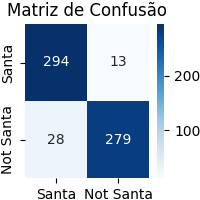
\includegraphics[scale=1]{tests/test2_3_e5b64class10_20231211_220722/confusion_matrix.png}
  \caption{Matriz de Confusão}
  \label{fig:fig03}
 \end{center}
\end{figure}

\begin{figure}[ht]
 \begin{center}
   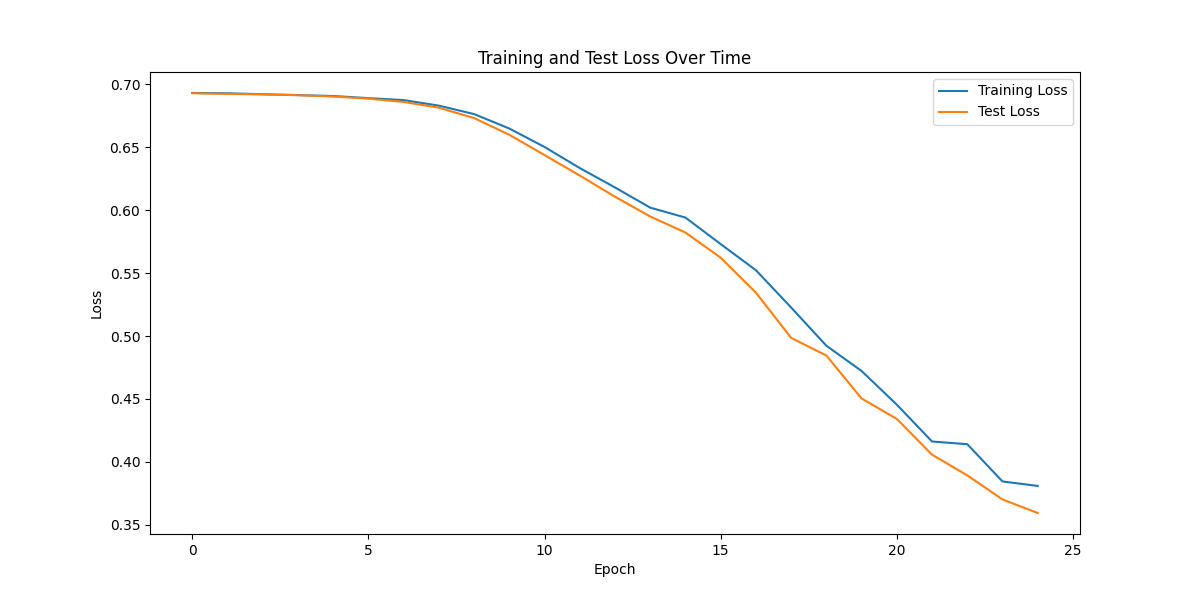
\includegraphics[scale=0.8]{tests/test2_3_e5b64class10_20231211_220722/loss_over_time.png}
  \caption{Gráfico de Perda}
  \label{fig:fig04}
 \end{center}
\end{figure}
